\documentclass[CMPE]{KGCOEReport}
\usepackage{float}
\usepackage{adjustbox}
\graphicspath{ {./images/} }

\newcommand{\name}{Mohammed Fareed \\ Trent Wesley}
\newcommand{\exerciseNumber}{5}
\newcommand{\exerciseDescription}{MSP432 Timers, Interrupts, and Analog-to-Digital
Converter}
\newcommand{\dateDone}{September 27, 2023}
\newcommand{\dateSubmitted}{October 18, 2023}

\newcommand{\classCode}{CMPE 460}
\newcommand{\LabSectionNum}{1}
\newcommand{\LabInstructor}{Prof.\ Hussin Ketout}
\newcommand{\TAs}{Andrew Tevebaugh \\  Colin Vo}
\newcommand{\LectureSectionNum}{1}
\newcommand{\LectureInstructor}{Prof.\ Hussin Ketout}


\begin{document}
\maketitle

\section*{Abstract}

\section*{Design Methodology}

Interrupts are a useful tool for efficiently handling events by pausing the CPU's current task to handle another. Interrupts provide the benefit of assigning priority to certain events so that they can be executed in a proper order. In addition, interrupts avoid the need to constantly poll, which can interfere with the flow of a program. Interrupts are used extensively in this exercise by timers, switches, UARTs, and GPIO.\\

The MSP432 contains two Timer32 modules for timing operations. Each module contains a counter which can be configured as a 16-bit or 32-bit down counter. In this exercise, C code was written so that pressing Switch1 on the MSP432 microcontroller board activates Timer32-1 which toggles LED1 every 0.5 seconds. To accomplish this, Switch1 was configured to generate interrupts on the falling edge of the button click. The interrupt from a button click starts the interrupt service routine for the switch's port. Within the ISR, the interrupt flag for Switch1 is checked to see if the interrupt came from it. If the interrupt was from Switch1, the state of Timer32-1 gets toggled and a boolean value tracking Timer32-1's state is updated. While Timer32-1 is active, it generates an interrupt every 0.5 seconds. Every interrupt triggers an ISR which checks the state of LED1 with a boolean variable and toggles both the variable and the LED state.\\

More code was written to track time between button presses and cycle an LED through a list of colors. Switch2 on the MSP432 microcontroller board was configured to generate interrupts when pressed. The ISR of Switch2 would first check its interrupt flag to make sure that the interrupt came from it. If Timer32-2 was not already running according to a boolean flag variable, a millisecond counter variable gets set to 0, LED2 gets set to the next color, and a color index variable gets updated. Timer32-2 generates an interrupt every millisecond and triggers an ISR which increments a millisecond counter. If Timer32-2 was running on a Switch2 press, LED2 gets turned off and the UART sends a message of how much time has elapsed based on the millisecond counter. \\

Analog to digital converters are essential for converting real-world data into computer readable digital signals. The MSP432's ADC was used to measure the voltage which varied as the resistance of a photocell changed with light intensity. The circuit in Figure \ref{fig:photocell} was constructed to measure this varying voltage.

\begin{figure}[H]
    \centering
    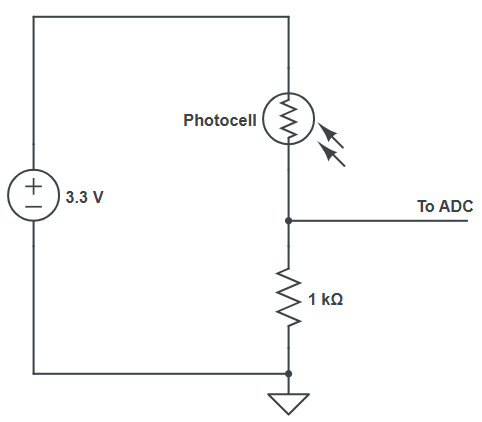
\includegraphics[width=0.4\textwidth]{photocellCircuit.png}
    \caption{Photocell Circuit}
    \label{fig:photocell}
\end{figure}

This circuit shown in Figure \ref{fig:photocell} is a voltage divider circuit with the middle node going to the ADC. The voltage at the middle node follows the behavior shown in Equation \ref{eq:voltageEq}.

\begin{equation}
\text{V}_\text{N} = 3.3\text{V} * \frac{1\text{k}\Omega}{1\text{k}\Omega + \text{R}_\text{Photocell}} \label{eq:voltageEq}
\end{equation}

Equation \ref{eq:voltageEq} shows that if the resistance of the photocell increases, the voltage measured by the ADC decreases. Since the resistance of photocell decreases with increased light intensity, it is known that the measured voltage will increase as light intensity increases.\\

To measure the voltage with the MSP432, the ADC needs to be initialized with C code. First, the reference was configured to be a static 2.5V. The code waits for the reference voltage to be ready by continually checking the variable reference voltage ready status register until it is set to 1. Then, the ADC's enable conversion bit within the control 0 register is set to allow programming. The code waits for the ADC to be ready by continually checking the control 0 register's busy status bit. Once the ADC is not busy, the code sets up the ADC to operate in single-channel, 14-bit resolution mode, with specific clock and pulse-mode configurations. Channel 6 is selected for conversion, and interrupts are disabled. Additionally, pin P4.7 is configured for analog input.\\

Timer32-1 was configured to generate interrupts every 0.5 seconds. With each interrupt, an interrupt service routine reads the value in the ADC memory register and outputs the value in decimal and hexidecimal. The voltage is calculated by multiplying the value by 2.5 since the reference range is 2.5V and dividing it by $2^{14}$ since a resolution of 14 bits is used. \\

The photocell was replaced with a TMP36 temperature sensor. Using the datasheet, it was found that the voltage output is a linear function of the temperature. The relation between the output voltage and the temperature in degrees celsius is shown in Equation \ref{eq:temperatureEq}.

\begin{equation}
\text{T}_{^\circ\text{C}} = 100\text{V}_\text{out} - 50
\label{eq:temperatureEq}
\end{equation}

After finding the temperature in degrees Celsius with Equation \ref{eq:temperatureEq}, the temperature in Fahrenheit can easily be found with a simple Celsius to Fahrenheit conversion.

\section*{Results and Analysis}

Part 1 of this exercise was to toggle LED1 every 0.5 seconds using Timer32-1. The code for this part was tested by pressing Switch1 on the MSP432 microcontroller board, and verifying that LED1 toggled every 0.5 seconds. The switch was then pressed again and the LED was verified to stop toggling. The second switch was tested in the same manner, verifying that the LED cycled through the colors red, blue, green, cyan, magenta, yellow, and white. Figure \ref{fig:part1} shows the UART output of the time elapsed between button presses.

\begin{figure}[H]
    \centering
    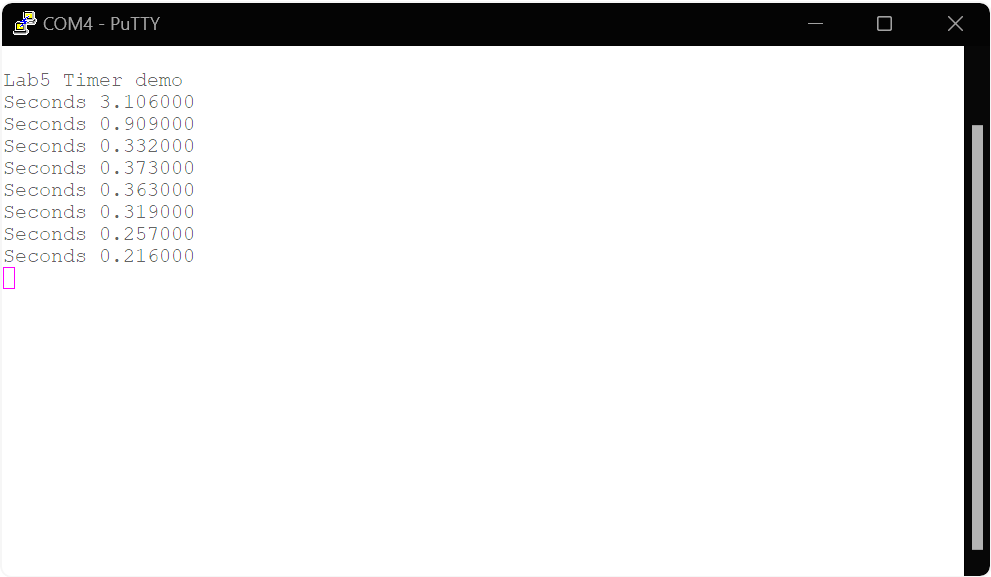
\includegraphics[width=0.75\textwidth]{part1.png}
    \caption{Part 1 UART Output}
    \label{fig:part1}
\end{figure}

The figure shows the time elapsed between button presses as the color of the LED changes back to red. The time between button presses was then verified by using the UART to print the time elapsed since the last button press, comparing the printed result with an external timer.\\

Part 2 of this exercise was to measure the voltage of a photocell using the ADC. The code for this part was tested by shining a flashlight on the photocell and verifying that the measured voltage increased. The measured voltage was then verified to decrease when the photocell was covered. Figure \ref{fig:part2a} shows the UART output of the measured voltage.

\begin{figure}[H]
    \centering
    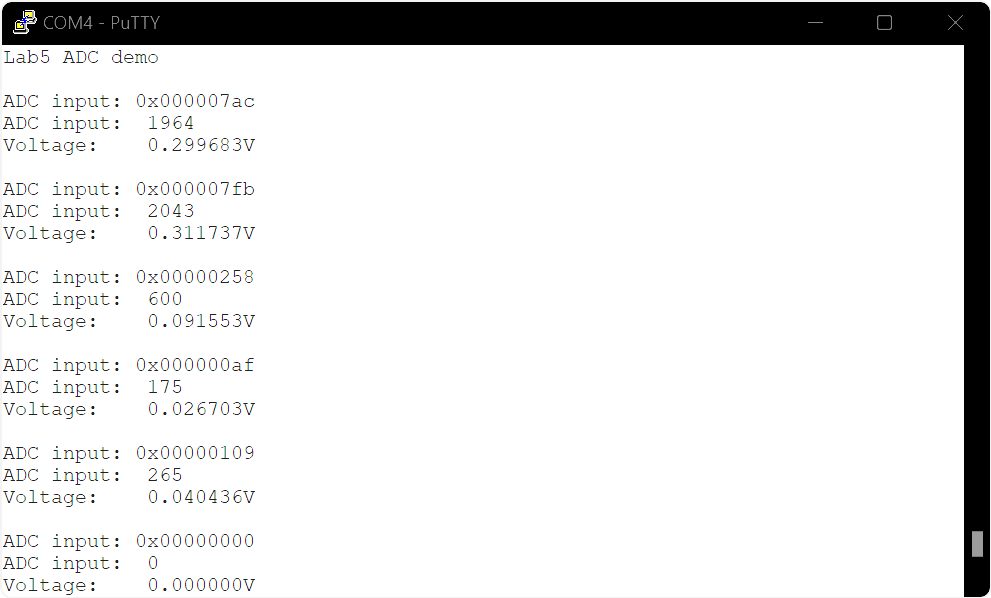
\includegraphics[width=0.75\textwidth]{part2a.png}
    \caption{Part 2 UART Output}
    \label{fig:part2a}
\end{figure}

The figure shows the measured voltage of the photocell as the light intensity changes. The measured voltage was then verified by using the UART to print the voltage, comparing the printed result with a multimeter. The result shows that the measured voltage when light was shined on the photocell was around 0.3V, and the measured voltage when the photocell was covered was 0V.\\

The code was then modified to use a temperature sensor, calculating the temperature from the voltage in both Celsius and Fahrenheit. Figure \ref{fig:part2b} shows the UART output after replacing the photocell with the temperature sensor TMP36.

\begin{figure}[H]
    \centering
    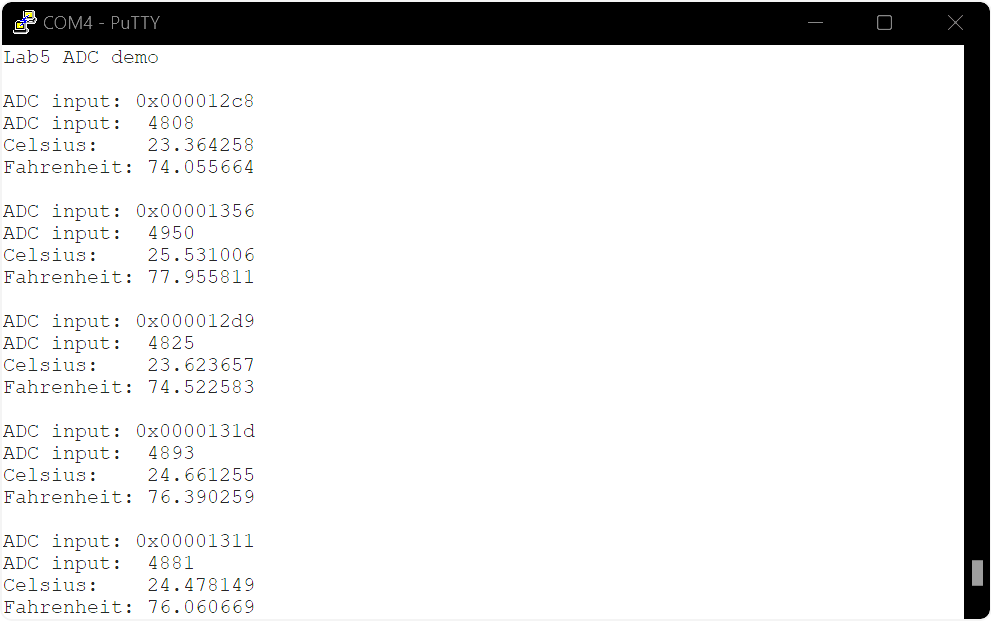
\includegraphics[width=0.75\textwidth]{part2b.png}
    \caption{Part 2 UART Output with TMP36}
    \label{fig:part2b}
\end{figure}

The figure shows the measured temperature of the sensor at room temperature, which was correctly around 24 degrees Celsius and 75 degrees Fahrenheit.\\

Part 3 of the exercise was to interface a line scan camera using timers and an ADC to send the received data serially over UART. The code for this part was tested by connecting the line scan camera to the MSP432 microcontroller board and verifying that the received data was sent correctly over UART using PuTTY.\\

The camera was then tested by pointing it at a bright light then a dark area repeatedly. The received data was then plotted using MATLAB to verify that the received data behaved correctly. The data was plotted raw, after being processed by a 5-points moving average filter, and after being converted to a binary image. The threshold used to convert the data to a binary image was then adjusted through trial and error to 5000. Figure \ref{fig:part3} shows the received data plotted in MATLAB.

\begin{figure}[H]
    \centering
    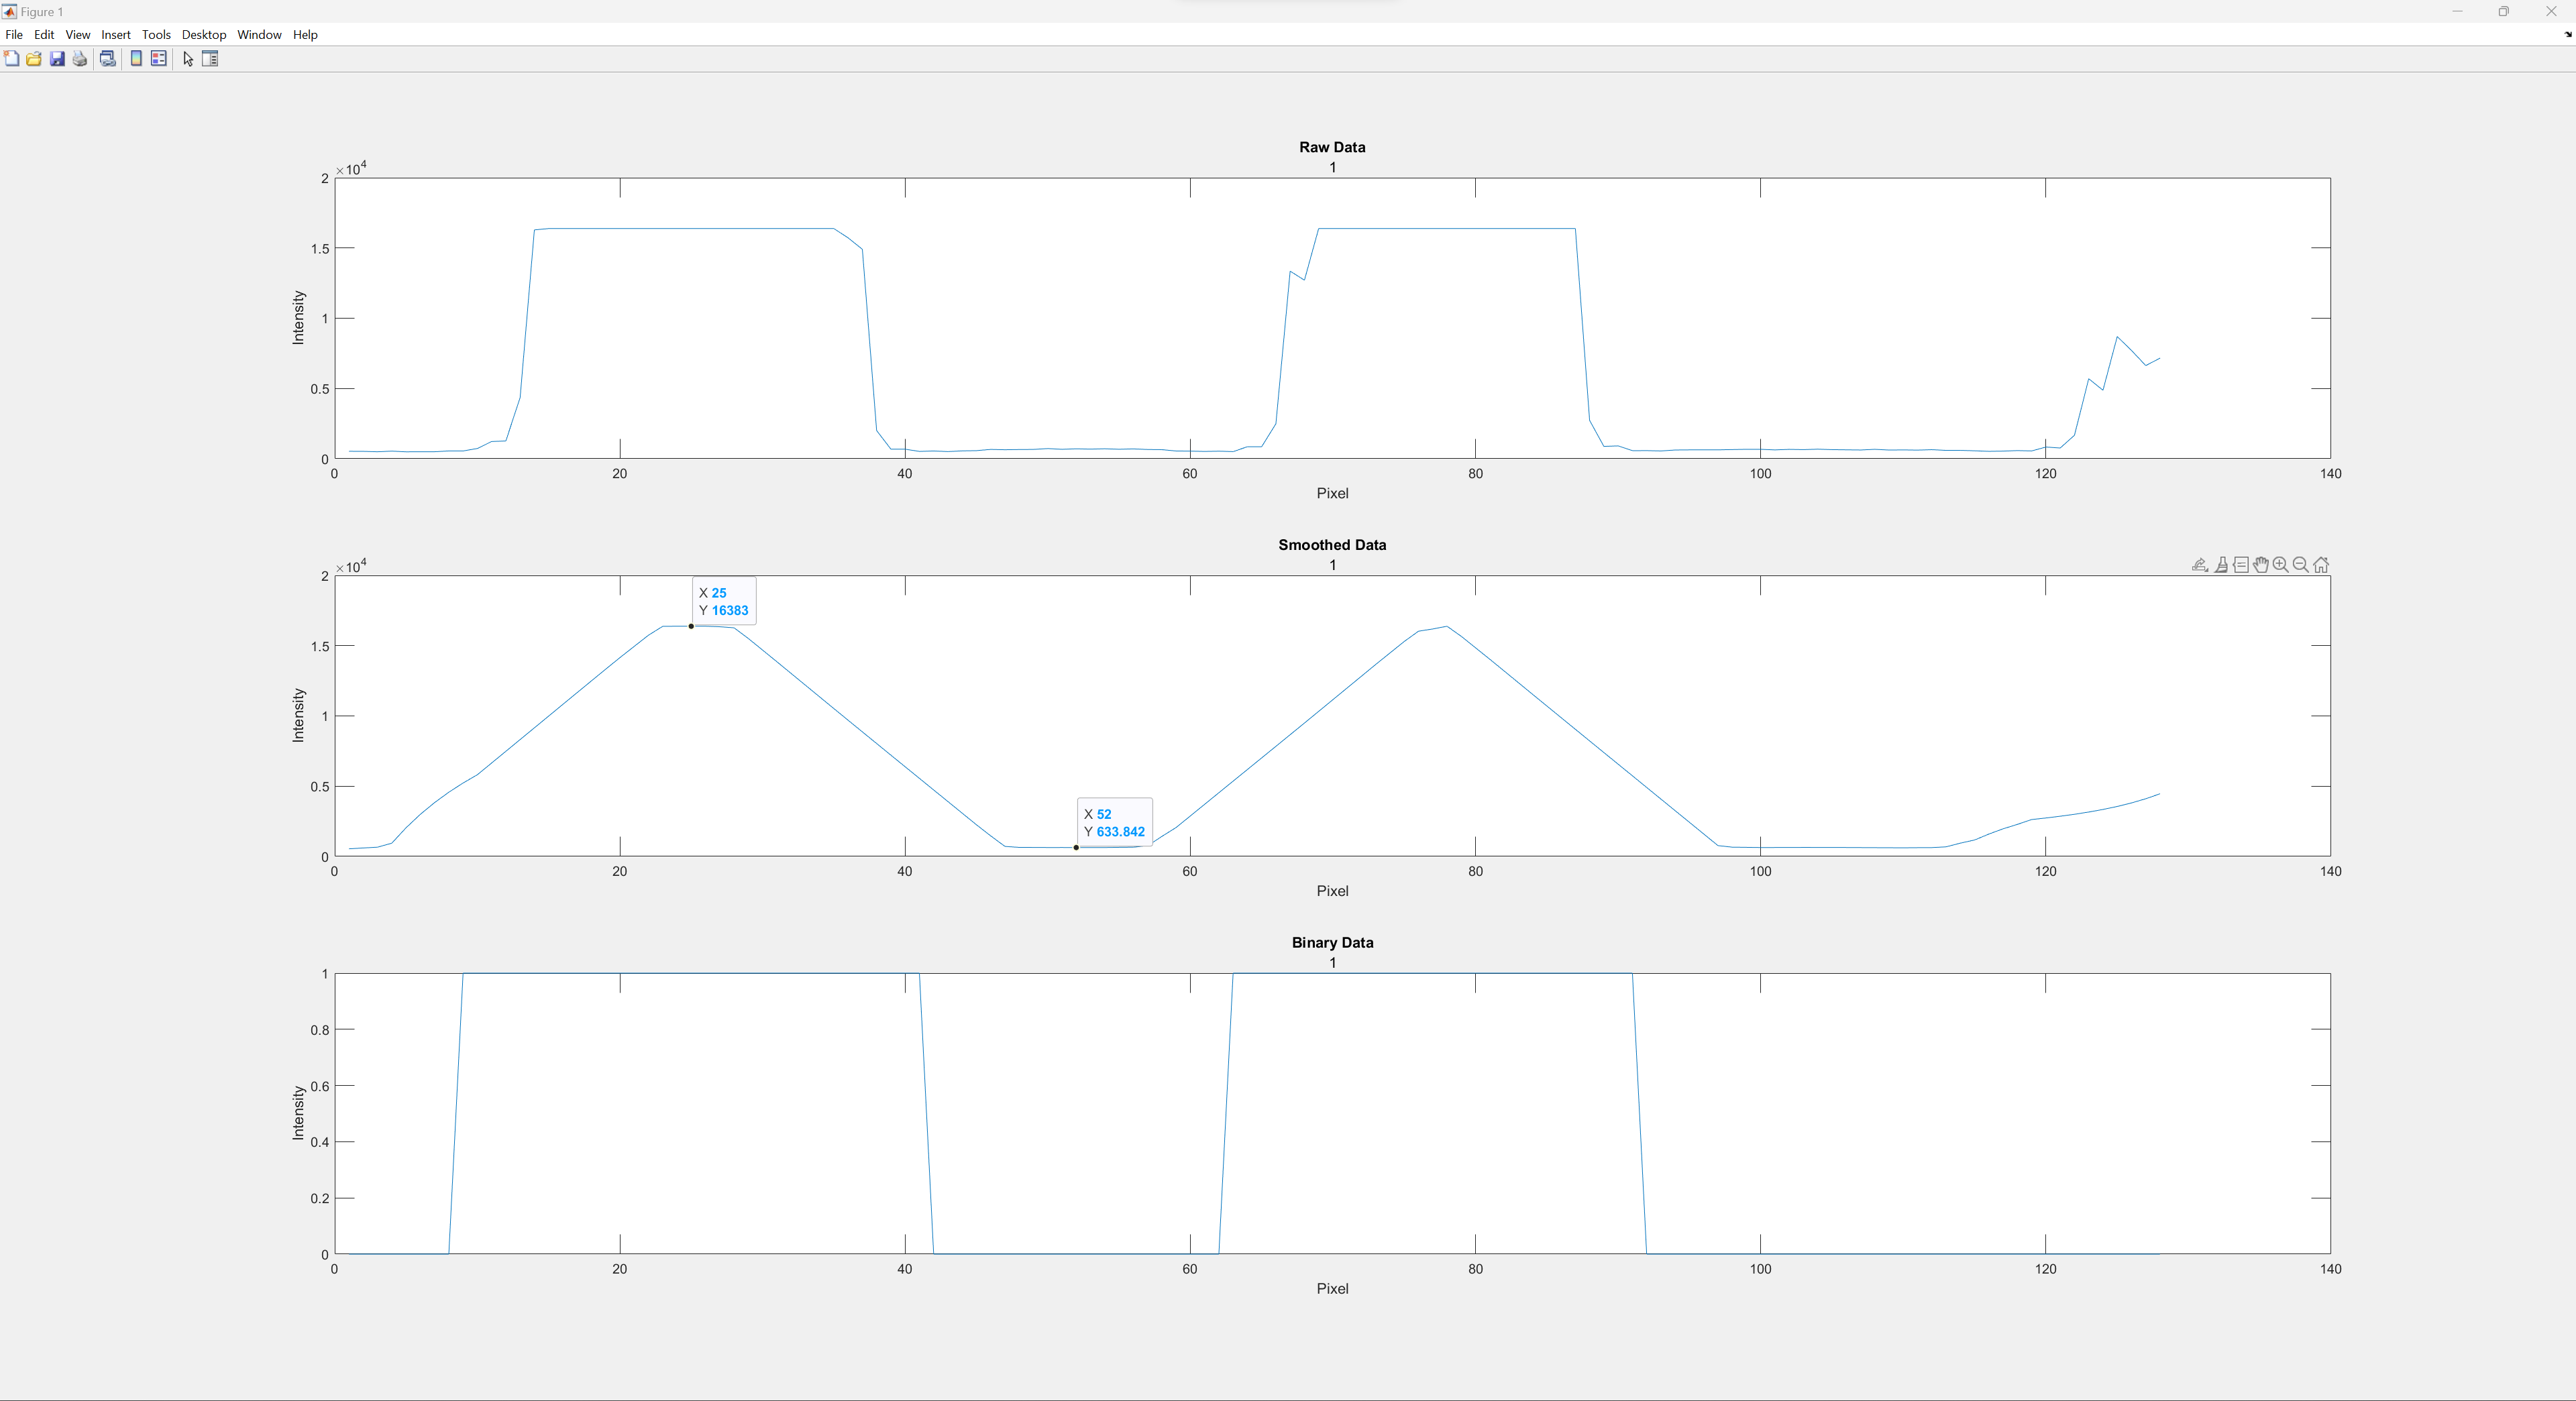
\includegraphics[width=1.00\textwidth]{part3.png}
    \caption{Part 3 MATLAB Plot}
    \label{fig:part3}
\end{figure}

The figure shows that the raw data correctly reflects the camera's output, with the dark area having a lower value than the bright area, creating a clock-like pattern. The figure also shows that the moving average filter correctly smooths the data, creating a triangular wave, gradually increasing and decreasing as the camera is moved from the bright area to the dark area. The figure also shows that the binary image correctly converts the data to a binary image, outputting a 1 for the bright area and a 0 for the dark area, which acts as an edge detector.\\

A sine wave was generated for part 4 of the exercise using MCP4901 DAC by interfacing it with the MSP432 microcontroller board using SPI using a reference voltage of 3.3 V. The code written for this part generated a 1 Hz sine wave spanning the possible outputs of the DAC. Figure \ref{fig:part4} shows the generated sine wave measured by an oscilloscope.

\begin{figure}[H]
    \centering
    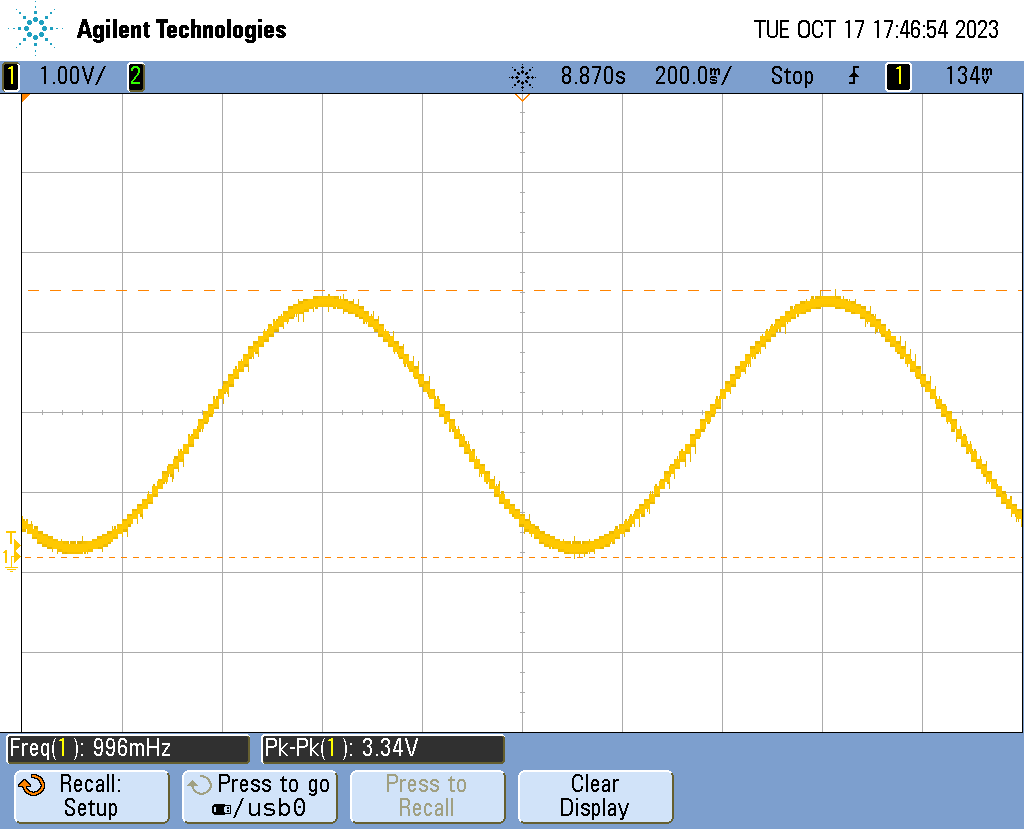
\includegraphics[width=0.75\textwidth]{part4.png}
    \caption{Part 4 Oscilloscope Output}
    \label{fig:part4}
\end{figure}

The figure shows the generated 1 Hz sine wave spanning the possible outputs of the DAC. The oscilloscope screen capture shows that the sine wave has a frequency of 0.996 Hz and a peak-to-peak voltage of 3.34 V.\\

The smallest amount of time that could be measured on the MSP432 depends on the frequency the board is running at. Since an interrupt can be generated on every clock cycle, the smallest amount of time that can be measured is the period of the clock. The MSP432 microcontroller board used in this exercise has a clock frequency of 48 MHz, so the smallest amount of time that can be measured is 20.83 ns. The longest amount of time that can be measured is arbitrary since an accumulator can be used to measure arbitrarily large amounts of time.\\


\section*{Questions}

\section*{Conclusion}

\newpage
\begin{figure}[H]
    \centering
    \begin{adjustbox}{center}
        
\includegraphics[width=1.26\textwidth]{signoff.pdf}
    \end{adjustbox}
\end{figure}

\end{document}
